\documentclass[11pt]{article}
\usepackage{mypackages}
\begin{document}

\maketitle

\section{Data}\label{Data}

To train and test our Actor-Critic and asynchronous advantage Actor-Critic implementation we will use
the OpenAI Gym framework\cite{openAIGym}.
This framework provides an interface to 118 Atari 2600 games,
that can be used by developers to compare and test their reinforcement learning algorithms.

 
In the Atari enviroments there is always a finite \textit{action space} and continous \textit{state space}.
The state space is continous because a \textit{state} is represented as a RGB image - a screenshot from a game
at the given time. The action space is finite because there is always a fixed amount of
actions available to the player in the OpenAI Gym framework.

Simulating an action in a game takes the player into a new state
and returns information about the new state,
the \textit{reward} the action trigered and a \textit{binary signal} which indicates whether the 
game is done or not.
The reward is the score gained from transitioning to the new state and
it is not uncommon for this reward to be $0$ as many of the players actions do not produce immediate rewards.
In most of the Atari games performing an action for a single frame have almost no impact,
so instead taking an action using the OpenAI Gym framework
results in that action being repeated $x$ times, where $x$ is uniformly sampled from $\{2, 3, 4\}$.

\subsection{Cart-Pole}

Among a lot of other game types OpenAI gym also supports an interface
to the Cart-Pole problem.
A player can win the Cart-Pole game if they manage to balance a pole connected to the top of a moving cart for
200 consecutive time steps.
The player loses if the pole moves more than 15 degrees from an upright position in
either direction or if the cart exits the frame.

\begin{figure}[!h]
    \centering
    \fbox{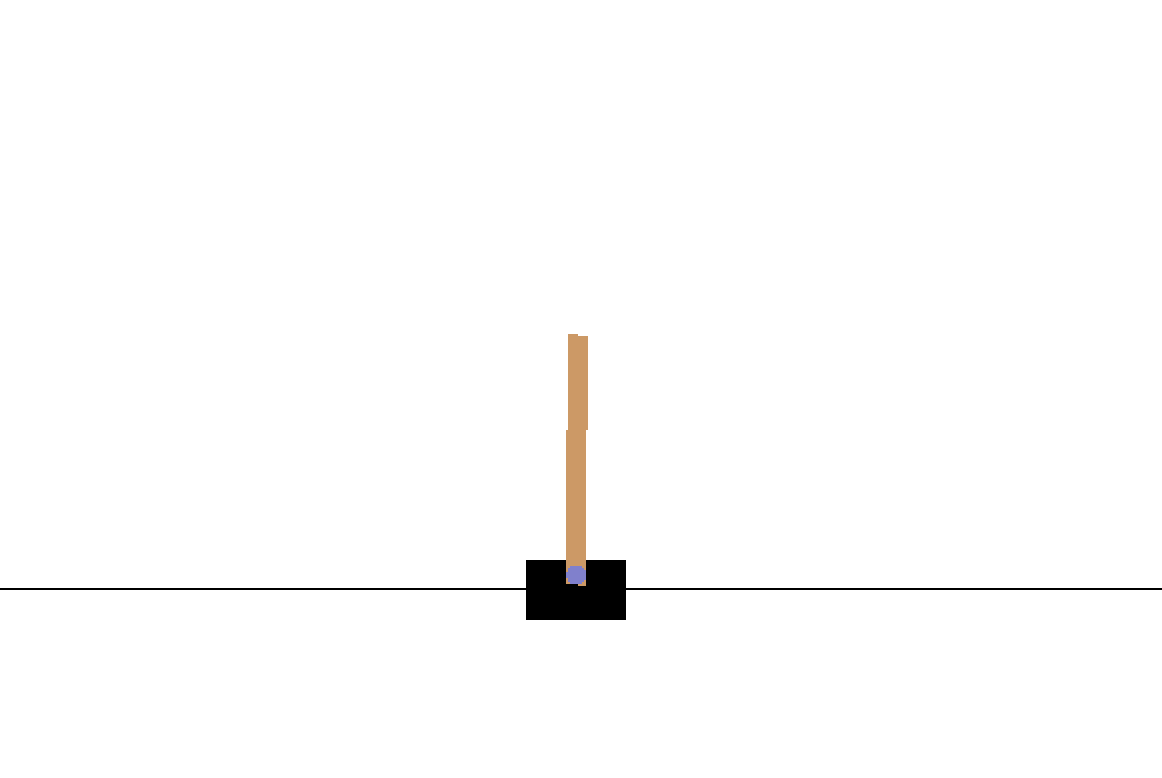
\includegraphics[scale=0.5]{include/cartpole.png}}
    \caption{A frame from Cart-Pole.}
    \label{fig:cartpole}
\end{figure}

Unlike the Atari environments a state in Cart-Pole consits of only four elements - the position and velocity of the cart, and the
angle and angular velocity of the pole.
Each time step, corresponding to a new frame, the player has to chose between moving the cart to the right or to the left and it is not possible
to do nothing.
For every time step the pole hasn't moved more than 15 degrees from the starting position and
the cart has stayed inside of the frame, the player is awarded a single point.

We will be using the Cart-Pole problem as a proof of concept for our Actor-Critic implementation and will
compare it to the A3C algorithm used on the same problem.
The reason for using the Cart-Pole problem is that it should be easier
to solve, because each state consists of fewer dimensions than a state
from an Atari game.


\subsection{Atari 2600 games}\label{sec:atari}

A state in an Atari game is represented as a 3-dimensional matrix representing a
frame.
This means that instead of only taking 4 elements into consideration when picking an action,
the player is now faced with a much more complex view. 
In general we want the learning agent to be able to pick an action from all
the available actions, but in some of the Atari games there are duplicate actions.
To speed up the training we have chosen to remove duplicates of the same action
from the action space.

All of the games have the same resolution of $210 \times 160$ pixels.
Each pixel contains three channels corresponding to the red, green and blue intensities of the pixel.
\begin{figure}[H]
    \begin{subfigure}{.3\textwidth}
        \centering
        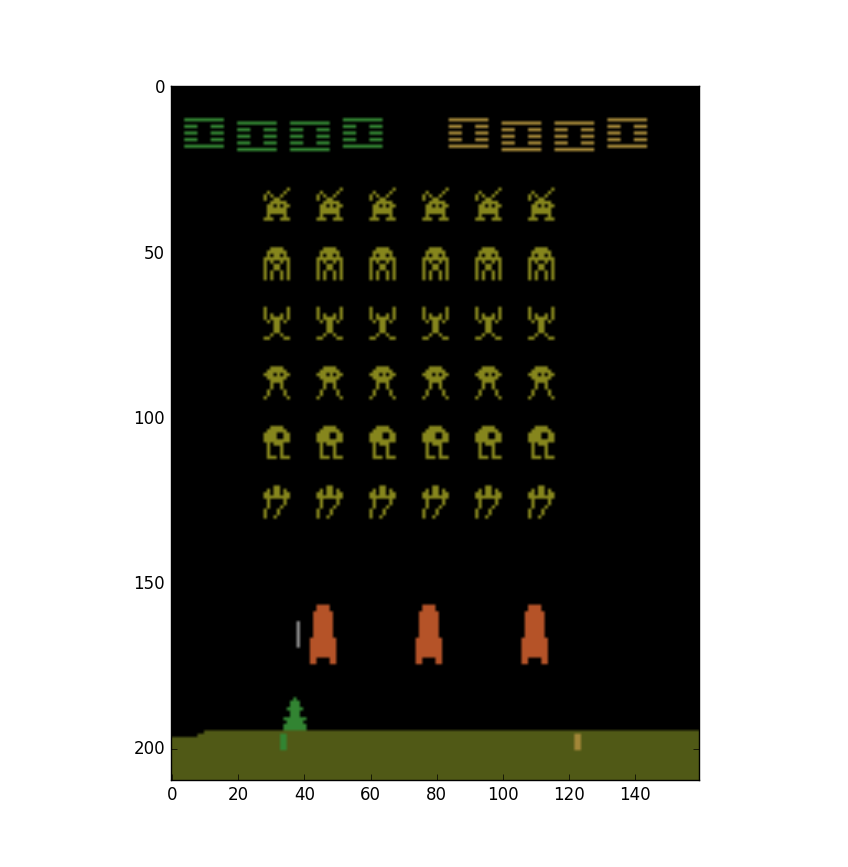
\includegraphics[scale=0.25]{include/space_invaders_1.png}
        \caption{Space Invaders.}
        \label{fig:scan}
    \end{subfigure}
    \begin{subfigure}{.3\textwidth}
        \centering
        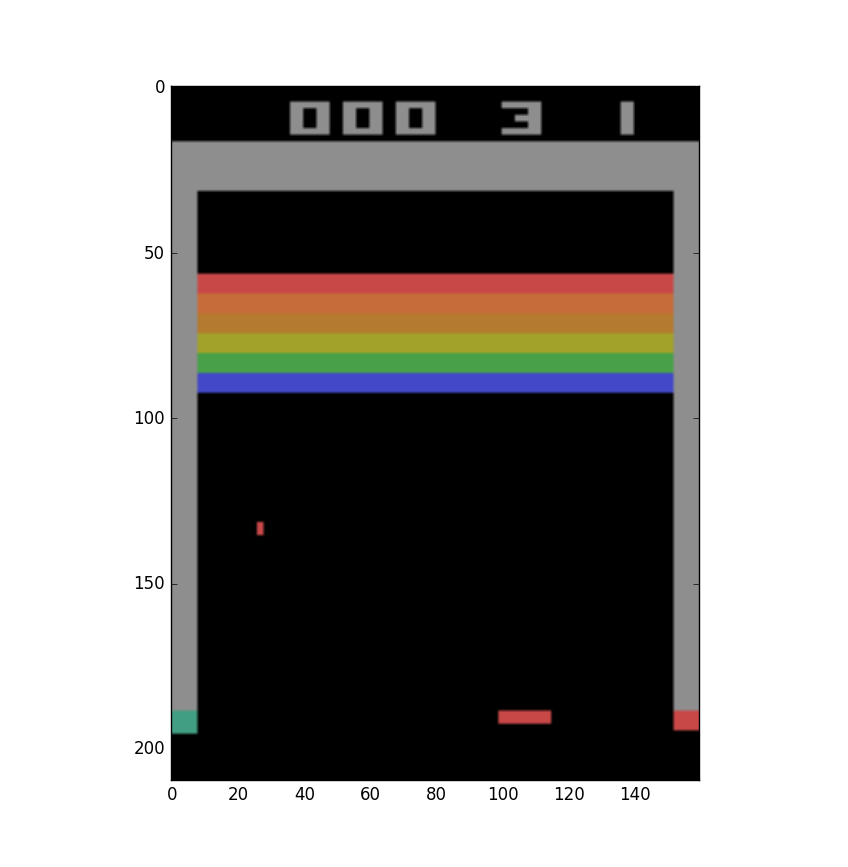
\includegraphics[scale=0.25]{include/breakout_1.png}
        \caption{Breakout.}
        \label{fig:scanlike}
    \end{subfigure}
    \begin{subfigure}{.3\textwidth}
        \centering
        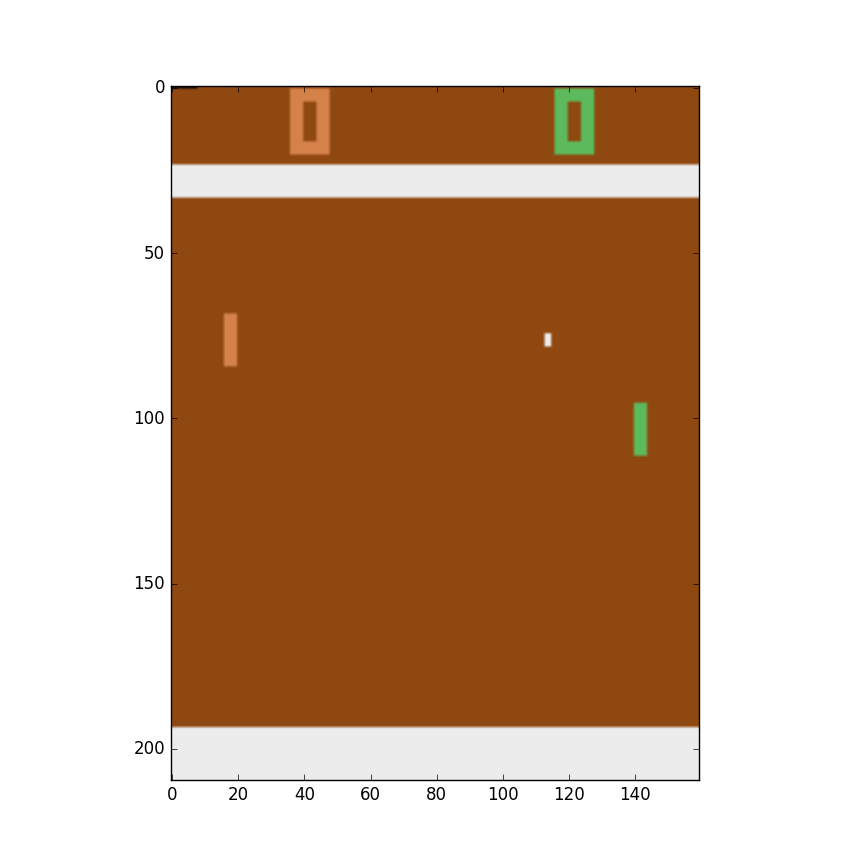
\includegraphics[scale=0.25]{include/pong_1.png}
        \caption{Pong.}
        \label{fig:scan}
    \end{subfigure}
    \caption{Frames from the Atari games we will be playing, before the preprocessing step is performed.}
     \label{fig:games}
\end{figure}
Using the raw Atari frames can be computationally demanding, so we have chosen
to preprocess our data as described in \cite{dqn}. 
The first step of the preprocessing is to reduce the amount of channels used to
represent the image.
We achieve this by taking the mean over the three channels, which results
in a naive grayscaling of the images.
\begin{figure}[H]
    \begin{subfigure}{.3\textwidth}
        \centering
        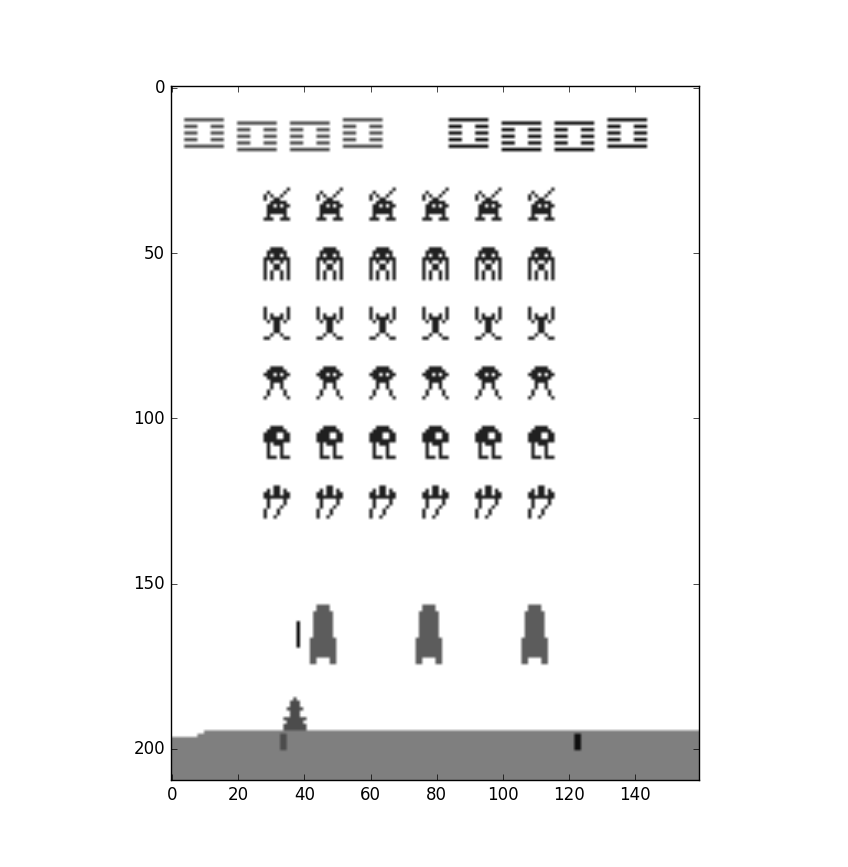
\includegraphics[scale=0.25]{include/space_invaders_1_gray.png}
        \caption{Space Invaders.}
        \label{fig:scan}
    \end{subfigure}
    \begin{subfigure}{.3\textwidth}
        \centering
        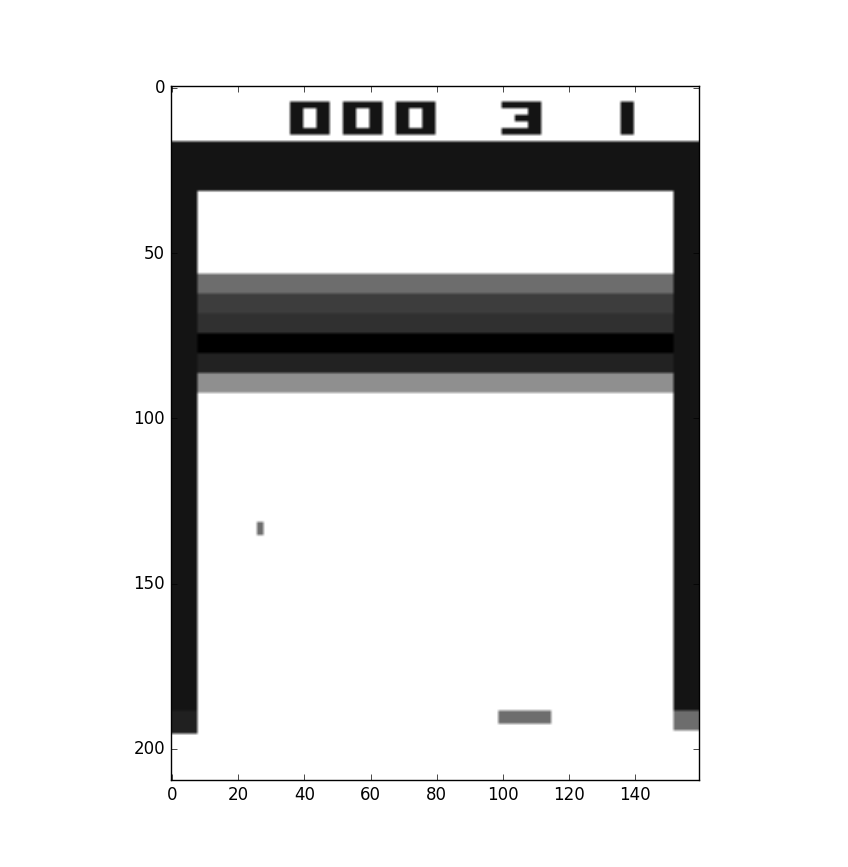
\includegraphics[scale=0.25]{include/breakout_1_gray.png}
        \caption{Breakout.}
        \label{fig:scanlike}
    \end{subfigure}
    \begin{subfigure}{.3\textwidth}
        \centering
        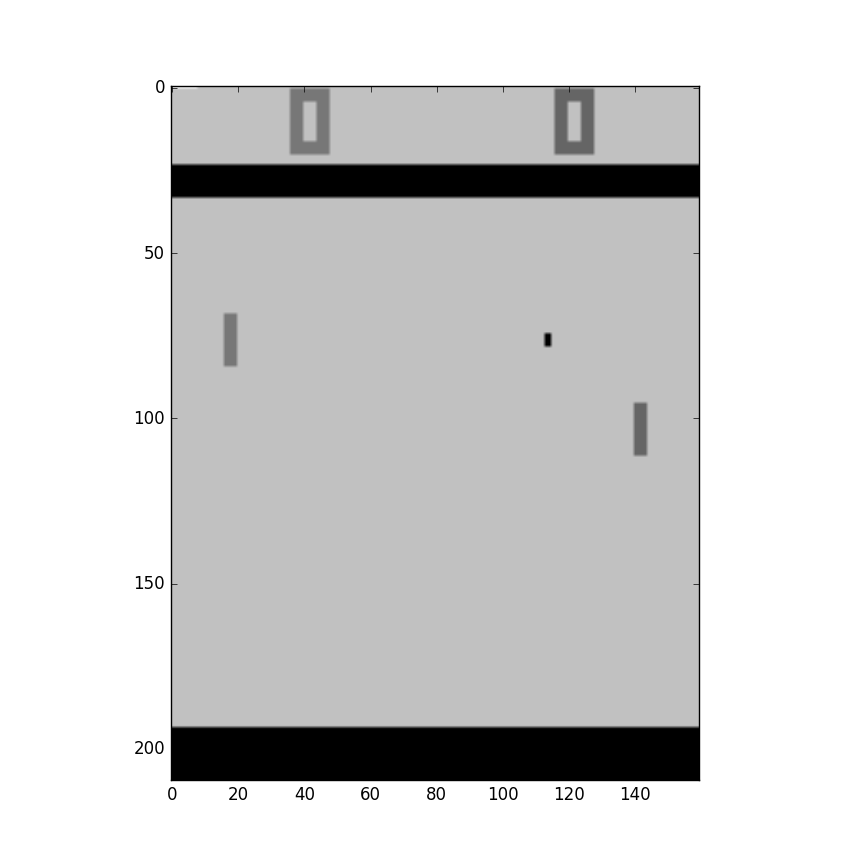
\includegraphics[scale=0.25]{include/pong_1_gray.png}
        \caption{Pong.}
        \label{fig:scan}
    \end{subfigure}
    \caption{The frames from \ref{fig:games} after being grayscaled.}
     \label{fig:grays}
\end{figure}

We further reduce the dimensions of the gray-scaled images
to $84 \times 84$ pixels, containing a single value.
The aim of this resized frame is to represent the game state
using fewer pixels, without losing information about the objects
in the frame.

\begin{figure}[H]
    \begin{subfigure}{.3\textwidth}
        \centering
        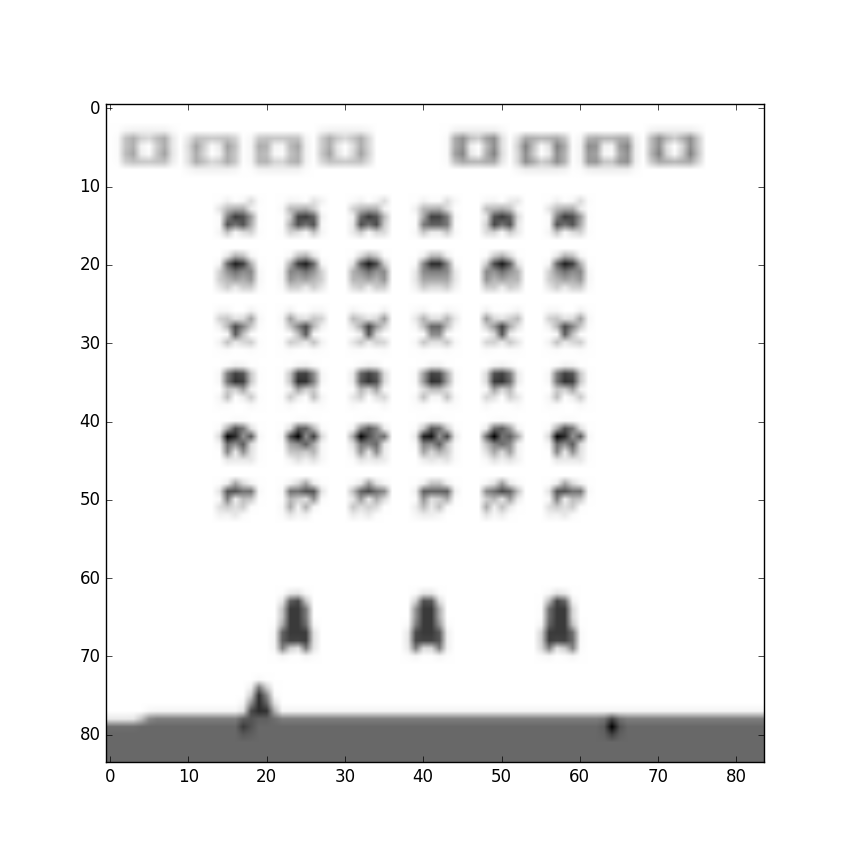
\includegraphics[scale=0.23]{include/space_invaders_1_gray_resized.png}
        \caption{Space Invaders.}
        \label{fig:scan}
    \end{subfigure}
    \begin{subfigure}{.3\textwidth}
        \centering
        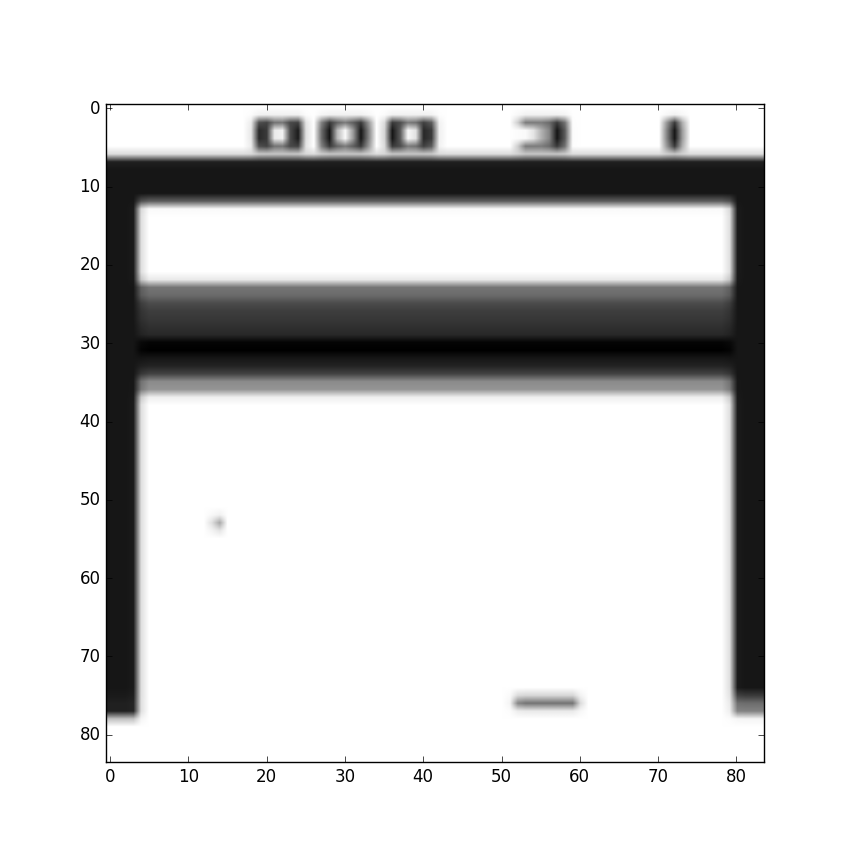
\includegraphics[scale=0.23]{include/breakout_1_gray_resized.png}
        \caption{Breakout.}
        \label{fig:scanlike}
    \end{subfigure}
    \begin{subfigure}{.3\textwidth}
        \centering
        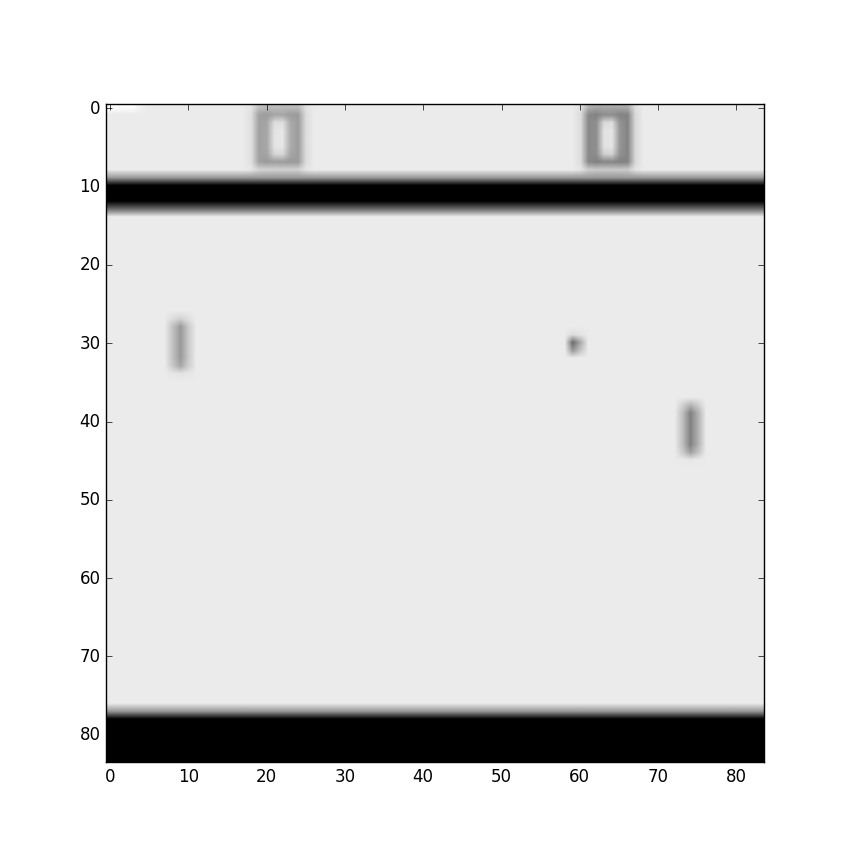
\includegraphics[scale=0.23]{include/pong_1_gray_resized.png}
        \caption{Pong.}
        \label{fig:scan}
    \end{subfigure}
    \caption{The grayscaled frames from \ref{fig:grays} resized.}
     \label{fig:rez}
\end{figure}

By preprocessing the data the remaining feature extraction becomes computationally 
cheaper, as the dimensions have been significantly reduced compared to the raw Atari RGB frames.

\end{document}
